% arara: lualatex: { synctex: yes, shell: yes } 
% arara: biber 
% arara: lualatex 
% if changed(toFile("ethik.bib")) || missing(toFile("ethik.bib"))

% LTeX: language=de-DE

% % -*- coding:utf-8 -*-
\documentclass[11pt, a4paper]{scrartcl}
\nonstopmode

% Basic Packages
%\usepackage[utf8]{inputenc}
%\usepackage[T1]{fontenc}
\usepackage[ngerman]{babel}

% Geometry
\usepackage[a4paper,
            bindingoffset=0.2in,
            left=1.5in,
            right=1.5in,
            top=1in,
            bottom=1in,
            footskip=.3in]{geometry}
            
% Textstuff
\usepackage{csquotes}
\usepackage{url}
\usepackage{hyperref}
\usepackage{lmodern}            % Provides the Latin Modern Font which offers more glyphs than the default Computer Modern
\usepackage[nameinlink]{cleveref}
\crefname{figure}{Abbildung}{Abbildung}
\crefname{subfigure}{Abbildung}{Abbildung}
\crefname{table}{Tabelle}{Tabelle}
\crefname{listing}{Quelltext}{Quelltext}
\crefname{chapter}{Kapitel}{Kapitel}
\crefname{section}{Abschnitt}{Abschnitt}
\crefname{subsection}{Abschnitt}{Abschnitt}
\crefname{subsubsection}{Abschnitt}{Abschnitt}
\crefname{beispiel}{Beispiel}{Beispiel}
\crefname{lemma}{Lemma}{Lemma}

% Set Paragraph Skip
\setlength{\parskip}{0.5\baselineskip}%
\setlength{\parindent}{0pt}%

% gfx
\usepackage{pgfpages}
\usepackage{svg}
\usepackage{graphicx}
\usepackage{xcolor}
\usepackage{color}
\usepackage{wrapfig}

% Tikz
\usepackage{tikz}
\usetikzlibrary{positioning,calc}

% Bibliography
\usepackage{biblatex}
\addbibresource{ethik.bib}




\title{Faites Vos Jeux}
\subtitle{So viele Daten sind das ja nicht... oder?}
\author{Etienne Palanga}
\date{\today}


\begin{document}

\maketitle

\tableofcontents

\begin{frame}{Datenschutz}
  \centering 
  
  \note[item]{Überall werden Daten erhoben}
  \note[item]{
    Manchmal eindeutig 
    \begin{itemize}
      \item Eingabe von Daten bei Kontoerstellung
    \end{itemize}
  }
  \note[item]{
    Aber viel öfter ohne wirkliches Wissen
    \begin{itemize}
      \item Tracker auf Websites
      \item Nutzung anderer Dienste
    \end{itemize}
  }
  \note[item]{
    Deswegen Datenschutz wichtig
  }

  
\includegraphics[width=0.45\textwidth]{images/computer_data_tobu} 
\end{frame}

\begin{frame}{Datenschutz}

  \note<1->[item]{Definition aus Paper von Lee et al. (meine Zusammenfassung u. Übersetzung)}
  \note<2->[item]{Schutz vor unauthorisiertem Zugriff}
  \note<3->[item]{Sicherung, dass die Daten angemessen genutzt werden}
  \note<4->[item]{Korrektheit und Vollständigkeit gesammelter Daten über Personen}
  \note<5->[item]{Verfügbarkeit der Daten für das Subjekt und die Sicherung der Rechte des Subjekts an seinen Daten}
  \note<6->[item]{Sicherung der Rechte des Subjekts die Daten einzusehen, aktualisieren oder korrigieren}

  Nach Lee et al.\cite{lee_ethical_2016}:

  \begin{block}{Datenschutz}
    \begin{itemize}
      \item<2->{Schutz vor unauthorisiertem Zugriff}
      \item<3->{Sicherung, dass die Daten angemessen genutzt werden}
      \item<4->{Korrektheit und Vollständigkeit gesammelter Daten über Personen}
      \item<5->{Verfügbarkeit der Daten für das Subjekt und das Besitzrecht des Subjekts an seinen Daten}
      \item<6->{Sicherung der Rechte des Subjekts die Daten einzusehen, aktualisieren oder korrigieren}
    \end{itemize} 
  \end{block}
\end{frame}

\begin{frame}{Datenschutz}
  \centering

  \note<1->[item]{Selbes Paper}
  \note<1->[item]{Gesetz und Ethik sind verbunden}
  \note<2->[item]{Gesetz gibt Ethik Durchsetzungsvermögen \begin{itemize}
      \item Bsp. Ethischer Schluss: Stehlen ist falsch
      \item Aber ohne Gesetz: keine Durchsetzung
    \end{itemize}
  }
  \note<3->[item]{Ethik gibt Gesetz Kontext \begin{itemize}
      \item Bsp. Arbeit in Niedriglohnländer auszulagern ist legal, aber ist es ethisch?
    \end{itemize}
  }
  \note<3->[item]{Ethische Ideen über Datenschutz werden im Gesetz umgesetzt.}
  \note<3->[item]{Sehen das später etwas mehr}

  \begin{tikzpicture}
    \node (law) {
\includegraphics[width=0.25\textwidth]{images/book_law}};
    \node[below = 0cm of law] (law-name) {Gesetz};
    \node[right = 4cm of law] (ethics) {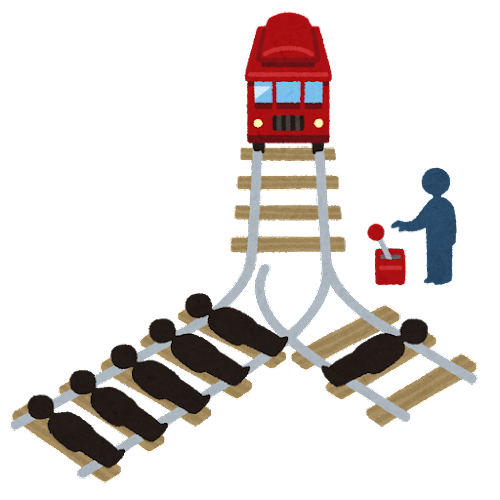
\includegraphics[width=0.25\textwidth]{images/trolley_problem}};
    \node[below = 0cm of ethics] (ethics-name) {Ethik};

    \draw<2->[-stealth] (law) to[out = 20, in = 160, edge node={node[above] {Kann durchsetzen}}] (ethics);
    \draw<3->[-stealth] (ethics) to[out = 200, in = 340, edge node={node[below] {Gibt Kontext}}] (law);
  \end{tikzpicture}

\end{frame}


\section{Grundlagen}

Zunächst wollen wir uns mit dem Zusammenhang von Gesetz und Ethik, sowie mit Datenschutz auseinandersetzen.
Ersteres ist wichtig für die spätere Evaluation des Fallbeispiels,
während Letzteres das Fundament für die Diskussion der Hauptthematik des Fallbeispiels bildet.

\subsection{Gesetz und Ethik}
\label{sec:02:lawethics}

\begin{wrapfigure}{r}{0.4\textwidth}
    \centering
    \begin{tikzpicture}[text node/.style={font=\sffamily\small}]
        \node (law) {
\includegraphics[width=0.25\textwidth]{images/book_law}};
        \node[text node, below = 0cm of law] (law-name) {Gesetz};
        \node[below = 3cm of law-name] (ethics) {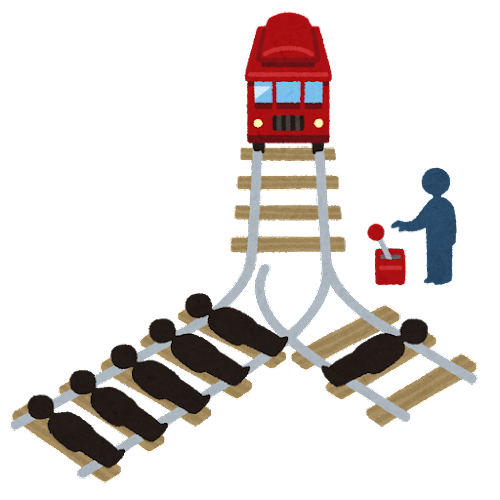
\includegraphics[width=0.25\textwidth]{images/trolley_problem}};
        \node[text node, below = 0cm of ethics] (ethics-name) {Ethik};

        \draw[-stealth, blue] (law) to[out = 300, in = 60, edge node={node[above left, text node] {\small Kann durchsetzen}}] (ethics);
        \draw[-stealth, red] (ethics) to[out = 120, in = 240, edge node={node[below right, text node] {\small Gibt Kontext}}] (law);
    \end{tikzpicture}
    \caption{Wechselwirkung von Gesetz und Ethik.}
    \label{fig:02:lawethics}
\end{wrapfigure}

So wie Privatsphäre, Sicherheit und Vertrauen verwandt sind, so sind es auch Ethik und das Gesetz.
Auf der einen Seite bietet das Gesetz einem ethischen Prinzip die Möglichkeit, 
das Prinzip tatsächlich in der Gesellschaft durchzusetzen.\cite{lee_ethical_2016}

Beispielsweise kann man aufgrund eines individuellen ethischen Verständnisses zu dem Schluss kommen, dass stehlen falsch ist.
Es ist natürlich auch so, dass die meisten Menschen dieses Verständnis im Allgemeinen teilen.
Allerdings ist das allein nicht genug, damit dieses Verständnis in der Gesellschaft auch durchgesetzt werden kann.
Denn einerseits kann es Menschen geben, die zwar dieses gleiche Verständnis besitzen, dies aber brechen.
Andererseits kann es auch sein, dass Menschen dieses Verständnis nicht teilen und aus diesem Grund stehlen.
Das Gesetz kann nun durch den Staat dieses Verständnis umsetzen, indem die,
die dieses Gesetz -- und damit das ethische Prinzip -- brechen, strafrechtlich verfolgt werden können.

Auf der anderen Seite bietet Ethik Kontext für bestehende Gesetze.
Ein Beispiel hierfür ist etwa das Auslagern von Arbeitsplätzen in ein Niedriglohnland.
Dies ist zwar hierzulande legal, allerdings lässt es sich streiten, ob dies ethisch korrekt ist.

Zudem existieren unbestimmte Rechtsbegriffe, wie hierzulande beispielsweise \enquote{Treu und Glauben} (zum Beispiel §~242 BGB).
Dieser sagt aus, dass man sich um dem jeweiligen Gesetz zu entsprechen \enquote{anständig und redlich verhalten} habe.\cite{alexy_treu_2019}
Wenn also festgestellt werden soll, ob eine Person entsprechend \enquote{Treu und Glauben} gehandelt hat,
können durchaus auch ethische Überzeugungen mit einfließen.

Diese Wechselwirkung ist in \cref{fig:02:lawethics} visualisiert.

Wie bereits in diesem Beispiel angedeutet, können Gesetze auch oft aus ethischen Überzeugungen entstehen.
Daher kann es bei der Evaluation ethischer Vertretbarkeit einer Handlung auch von Nutzen sein,
die gesetzliche Lage zu betrachten, sollten die zugrundeliegenden ethischen Überzeugungen erkennbar sein.

\subsection{Privatsphäre, Sicherheit und Vertrauen}

\begin{wrapfigure}{l}{0.6\textwidth}
    \centering
    \begin{tikzpicture}[text node/.style={font=\sffamily\small}]
        \node at (30:3cm) (privacy) {
\includegraphics[width=0.15\textwidth]{images/secret}};
        \node[text node, below = 0cm of privacy] (privacy-name) {Privatsphäre};
        \node at (150:3cm) (security) {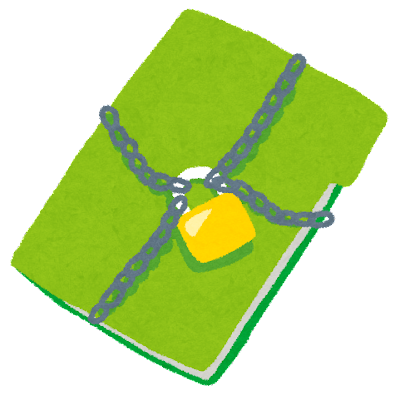
\includegraphics[width=0.15\textwidth]{images/lock_file}};
        \node[text node, below = 0cm of security] (security-name) {Sicherheit};
        \node at (270:3cm) (trust) {
\includegraphics[width=0.15\textwidth]{images/handshake}};
        \node[text node, below = 0cm of trust] (trust-name) {Vertrauen};
        
        \draw[stealth-stealth] (privacy) edge[bend right] node [text node, above] {Bedingen einander} (security);
        \draw[-stealth] (security-name) edge[bend right] node [text node, left] {\small Benötigt} (trust);
        \draw[stealth-] (trust) edge[bend right] node [text node, right] {Benötigt} (privacy-name);
    \end{tikzpicture}
    \caption{Wechselwirkungen von Sicherheit, Privatsphäre und Vertrauen.}
    \label{fig:02:secprivtru}
\end{wrapfigure}

Ebenfalls beschreiben Lee et al., dass die Gewährleistung von Privatsphäre und Sicherheit
eng mit dem Vertrauen in Dritte auch eine Wechselwirkung haben.\cite{lee_ethical_2016}
Soll die Privatsphäre einer Person geschützt, oder die Sicherheit einer Person garantiert werden, insbesondere durch Dritte,   
so muss Vertrauen in diese Dritten herrschen.

In beiden Fällen muss den Dritten Zugang zu dem privaten Bereich der Person gegeben werden.
Soll im Fall von Privatsphäre beispielsweise eine andere Person das eigene Tagebuch verwahren,
so muss das Vertrauen in diese andere Person herrschen, dass diese nicht selbst unerlaubt in dem Tagebuch liest.
Im Allgemeinen muss man Anderen vertrauen können, sollte man diesen Zugriff auf einen privaten Bereich geben. 

Im Falle Sicherheit muss zum Beispiel ein Bodyguard nah bei der zu beschützenden Person bleiben.
Dabei muss natürlich das Vertrauen herrschen, dass der Bodyguard selbst keine schlechten Absichten hat.
Allgemeiner, muss einem \enquote{Anbieter} von Sicherheit vertraut werden, dass dieser seine Arbeit gut und gewissenhaft tut.

Diese Zusammenhänge sind in \cref{fig:02:secprivtru} visualisiert.

Diese Aspekte finden sich im Datenschutz ebenfalls wieder.

\subsection{Datenschutz}

Datenschutz befasst sich mit dem Umgang mit den privaten Daten eines Subjekts.
Dazu zählt etwa wie auf diese zugegriffen werden darf, wie sie gesammelt werden dürfen oder von einer dritten Partei genutzt werden dürfen.
Besondere Wichtigkeit haben hier die Rechte, die das Subjekt selbst an ihren eigenen Daten hat.
Die Hauptaspekte lassen sich folgendermaßen zusammenfassen:\cite{lee_ethical_2016}  

\begin{center}
\parbox{0.9\textwidth}{
    Eine Instanz, die Daten Anderer verwaltet und Datenschutz betreibt, muss folgendes gewährleisten: 
    \begin{itemize}
        \item Schutz vor unauthorisiertem Zugriff
        \item Sicherstellen angemessener Benutzung der Daten
        \item Richtigkeit und Vollständigkeit gesammelter Daten über Personen oder Firmen
        \item Verfügbarkeit der Daten für das Subjekt und das Recht des Subjekts die Daten zu besitzen
        \item Das Recht des Subjekts, die Daten zu inspizieren, zu aktualisieren oder zu korrigieren
    \end{itemize}
}
\end{center}

Solange die Daten allein in der Hand ihres Eigentümers oder Eigentümerin sind, ist kein Datenschutz vonnöten,
da es hier unstrittig ist, ob auf die Daten zugegriffen werden darf oder ob sie verwendet werden dürfen.
Wir befassen uns also damit, was gelten soll, wenn die Daten in die Hände Anderer übergeben werden.

Wie wir bereits gesehen haben, hängen Privatsphäre, Sicherheit und Vertrauen zusammen. 
Dies ist auch bei Datenschutz nicht anders. Denn all diese drei Aspekte sind für Datenschutz nötig.
Durch den Schutz der privaten Daten des Subjekts wird dessen \emph{Privatsphäre} gewahrt.
Darüber hinaus muss die Daten schützende Instanz, die Daten in Hinblick auf die oben genannten Aspekte \emph{absichern}.
Die Instanz, die dies durchführt, benötigt das \emph{Vertrauen} dies gewissenhaft durchzuführen.

\subsubsection{Konsequenzen mangelnden Datenschutzes}

Natürlich ist Datenschutz aus dem Grund nötig, dass das Nicht-Schützen von Daten negative Konsequenzen mit sich zieht.
Dementsprechend muss sich Datenschutz auch mit diesen befassen, damit solche negativen Konsequenzen nach Möglichkeit vermieden oder zumindest vermindert werden können.
Nach Lee et al. lassen sich diese Konsequenzen in sogenannte \emph{Soft Costs} und \emph{Hard Costs} aufteilen. \cite{lee_ethical_2016}

Dabei handelt es sich bei Hard Costs um materielle Konsequenzen, wie finanzielle oder durch strafrechtliche Verfolgung entstehende Kosten.

Soft Costs sind dabei andere Konsequenzen, wie zum Beispiel der Verlust des Vertrauens der Kunden oder der Verlust eines guten Rufs.

\paragraph*{Facebook Datenleck 2021}

Ein Beispiel für solche negativen Konsequenzen ist ein Datenleck bei Facebook\footnote{\url{https://www.facebook.com/}}, 
der im Jahr 2021 entdeckt wurde.\cite{holmes_533_2021}
Hier wurden in 2021 die Daten von über \emph{533 Millionen} Nutzern und Nutzerinnen veröffentlicht.
Diese Daten beinhalten die Facebook IDs, Namen, Wohnorte, Geburtsdaten und weitere private Daten.
Nach Aussage von Facebook konnten die Daten aufgrund einer Sicherheitslücke in 2019 von Facebook erhoben werden.\cite{clark_facts_2021}

Die Veröffentlichung solcher Datensätze kann Identitätsdiebstahl vereinfachen.
Böswillige Parteien können mithilfe dieser Daten andere Personen imitieren um so potentiell an weitere persönliche Daten zu gelangen.

Zu diesem Vorfall sagte Alon Gal, der technische Direktor des Cyberkriminalität-Intelligenz-Unternehmens Hudson Rock\footnote{\url{https://www.hudsonrock.com/}} (übersetzt):
\blockquote[\cite{holmes_533_2021}]{
    Individuen, die sich bei einem reputablen Unternehmen wie Facebook registrieren, vertrauen ihnen mit ihren Daten
    und Facebook sollte mit den Daten mit höchstem Respekt umgehen. [\dots] 
    Dass die persönlichen Daten von Nutzern geleakt wurden, ist ein riesiger Vertrauensbruch und sollte auch so behandelt werden.
}

Auch aus diesem Zitat sehen wir, dass die Themen Vertrauen, Privatsphäre und Sicherheit sehr große Bedeutung für Datenschutz haben. 

Obwohl die genaue Wahrnehmung von Privatsphäre sich etwas von Kultur zu Kultur unterscheiden mag,
gibt es einen groben Konsens, dass Privatsphäre ein wichtiges, sozial vorteilhaftes Gut ist.\cite{lee_ethical_2016}

Zum Thema Datenschutz betrachten wir nun das Fallbeispiel \enquote{Faites Vos Jeux}\cite{kees_faites_2017} aus dem Informatik Spektrum 2017.


\section{Faites Vos Jeux}

\section{International Data Privacy Principles}

\section{DSGVO}

\newpage

\section{Quellen}

Alle verwendeten Illustrationen stammen von Irasutoya.\cite{mifune_irasutoya_nodate} 

\nocite{mifune_irasutoya_nodate}

\printbibliography[heading=none]


\end{document}
